\begin{figure}[h]
	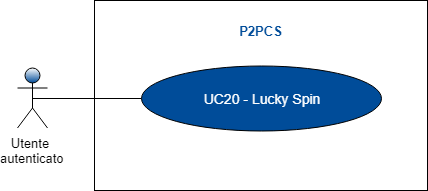
\includegraphics[width=9cm]{res/images/UC20Luckyspin.png}
	\centering
	\caption{UC20 - Lucky spin}
\end{figure}
\subsubsection{UC20 - Lucky spin}
\begin{itemize}
	\item \textbf{Attori Primari}: utente autenticato;
	\item \textbf{Descrizione}:	l'utente può visualizzare la lista dei premi ottenibili tramite la Lucky Spin\glo. Se è trascorso l'ammontare di tempo imposto dallo sviluppatore, può usare la Lucky Spin per ottenere un premio. Se non fosse interessato in quel momento a girare la ruota, può farlo in un secondo momento cliccando sul pulsante all'interno del Minigioco;
	\item \textbf{Scenario principale}: l'utente preme il pulsante \textit{Lucky Spin} all'interno del Minigioco. Nel caso sia trascorso il tempo imposto, può usare la Lucky Spin per ottenere un premio. I premi ottenibili sono del seguente tipo:
	\begin{itemize}
		\item accessori per personalizzare l'auto nel Minigioco;
		\item punti esperienza bonus;
		\item vincita di un viaggio gratuito con \textit{GaiaGo};
		\item buono sconto su un sito di e-commerce.	
	\end{itemize}
	\item \textbf{Precondizione}: l'utente ha premuto il pulsante della Lucky Spin nel Minigioco;
	\item \textbf{Postcondizione}: l'utente sta visualizzando la lista dei premi ottenibili tramite la Lucky Spin.
\end{itemize}
\subsubsection{UC21 - Vincita premio lucky spin}
\begin{figure}[h]
	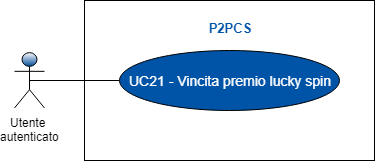
\includegraphics[width=9cm]{res/images/uc21.png}
	\centering
	\caption{UC21 - Vincita premio lucky spin}
\end{figure}
\begin{itemize}
	\item \textbf{Attori Primari}: utente autenticato;
	\item \textbf{Descrizione}: l'utente ha aspettato il tempo necessario e può usare la Lucky Spin\glosp per ottenere un premio;	
	\item \textbf{Scenario principale}: l'utente visualizza la schermata della Lucky Spin, nella quale può premere il pulsante \textit{Gira} per usare i suoi tentativi disponibili. Il premio gli verrà mostrato tramite un pop-up che metterà in risalto il premio vinto;
	\item \textbf{Precondizione}: l'utente autenticato ha aspettato il tempo necessario e ha usato la Lucky Spin;
	\item \textbf{Postcondizione}: l'utente autenticato ha vinto e ritirato il premio dalla Lucky Spin.
\end{itemize}
